\documentclass[../main.tex]{subfiles}
\graphicspath{{\subfix{../assets/}}}

\begin{document}

\section{\emph{A Simple Multi-Processor Computer Based on Subleq}}
\acrshort{subleq} nu e singurul limbaj sau arhitectură care face parte din categoria \acrshort{oisc}
dar e probabil cel mai popular și mai comun întâlnit în diferite lucrări. Alte variante
asemănătoare includ \emph{\acrfull{addleq}}, care e la fel ca \acrshort{subleq} dar folosește operația
de adunare și \emph{\acrfull{p1eq}} care folosește operația de incrementare cu 1.

În lucrarea \cite{subleqcpu} autorii profită de simplitatea arhitecturii pentru a dezvolta în \acrshort{vhdl} un procesor
multi-core care, cel puțin în teorie poate să aibă un număr nelimitat de core-uri. Placa folosită, menționată in lucrare,
este \emph{Altera Cyclone III EP3C16}, o placă de cost redus și cu resurse limitate. Avănd în vedere capacitatea de
memorie bloc valabilă pe placă, s-a estimat că e posibilă rularea a 28 de core-uri, fiecare cu o memorie cache de 2KB
sau 56 de core-uri cu doar 1KB memorie cache individuală. Placa va fi programată și conectată la un calculator printr-un
cablu USB după cum se vede în figura \ref{fig:simple_subleq_cpu_conn}.

\begin{figure}[h]
    \centering
    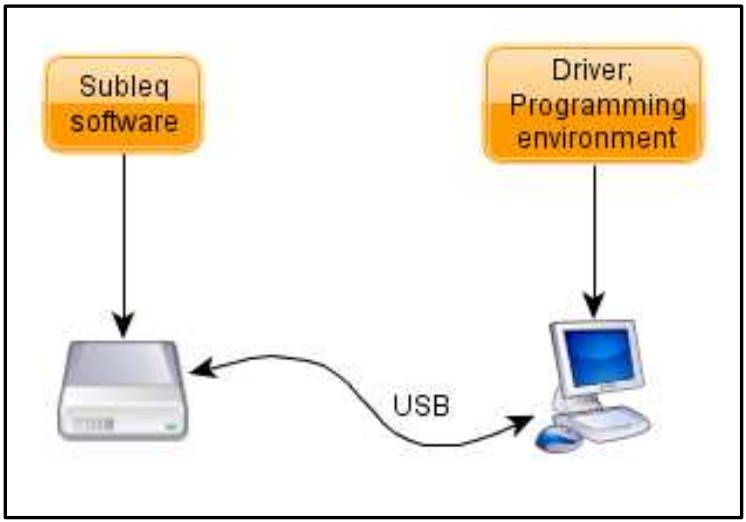
\includegraphics[width=0.8\textwidth]{simple_subleq_cpu_conn}
    \caption{Diagramă a conexiunilor extrasă din \cite{subleqcpu}}
    \label{fig:simple_subleq_cpu_conn}
\end{figure}

Deoarece este foarte puțina memoria pe placă, este necesară o memorie externă care să acționeze drept RAM/ROM.
Aici intervine calculatorul conectat la placă. Protocolul de comunicare \acrshort{spi} este folosit pentru a
facilita o comunicare stabilă între cele 2 dispozitive, astfel \emph{controller}-ul de memorie poate încărca
instrucțiuni și date din memoria calculatorului în memoria cache construită pe placă, făcând-o accesibilă
procesorului. Schema bloc este prezentată în figura \ref{fig:simple_subleq_cpu_block_diagram}.

\begin{figure}[h]
    \centering
    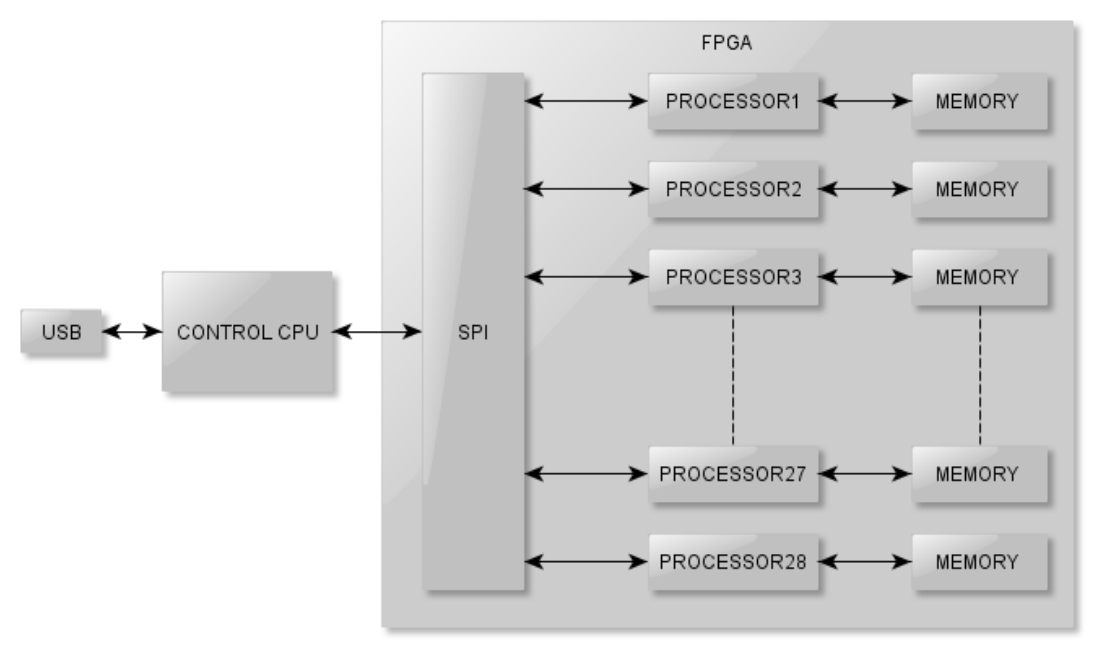
\includegraphics[width=0.8\textwidth]{simple_subleq_cpu_block_diagram}
    \caption{Diagramă bloc extrasă din \cite{subleqcpu}}
    \label{fig:simple_subleq_cpu_block_diagram}
\end{figure}

Scopul final este acela de a compara performanța arhitecturii \acrshort{subleq} cu altele care sunt folosite în industrie.
Pentru a face acest lucru este necesară o metodă eficientă de a scrie cod care să fie compilat în instrucțiuni ce
pot fi executate de procesor. Aceleași programe pot fi scrise ulterior într-un alt limbaj, precum C/C++, și rulate
pe un dispozitiv cu procesor \acrshort{cisc}. În capitolul 2 este prezentat pe scurt sintaxa limbajului de asamblare
conceput de ei. În capitolul 4 este descris un limbaj simplu, cu sintaxă asemănătoare cu C, care va fi folosit pentru
scrierea programelor. Fiecare subcapitol explică implementarea câte unui mecanism al limbajului, cât și codul aferent
în limbaj de asamblare. Acestea sunt:
\textit{
\begin{itemize}
    \item Stack
    \item Expressions
    \item Function calls
    \item Stack variables
    \item Multiplication
    \item Conditional jump
\end{itemize}}

Rezultatele arată că, deși are o performanță mult mai scăzută, un procesor \acrshort{oisc} este fezabil,
consumă puține resurse și are o viteză comparabilă cu procesoare mult mai complexe, atunci când numărul de core-uri e
suficient de mare.

\clearpage
\section{Inkel$^{TM}$ Pentwice Multicore Processor}
Un procesor single-core e considerabil mai simplu decât un procesor multi-core. Chiar și efortul depus în construirea
unui procesor cu doar 2 core-uri e mult mai mare. Acest lucru se datorează unui număr de factori, cum ar fi accesul
la memorie și coerența memoriei cache. Totuși vine cu promisiunea că totul e scalabil pănâ la un anumit număr foarte
mare de core-uri unde apar alte probleme. Deci în teorie nu există diferență între 2, 32 sau 1000 de core-uri, din punct
de vedere al efortului depus. În practică când ajungem la ceva atât de mare ca 1000 sau chiar și 100 lucrurile devin
mai complicate.

În lucrarea \cite{inkel} putem observa modificările care au fost făcute asupra procesorului \emph{Inkel Pentium}, dezvoltat
de aceeasi echipă, pentru a-l transforma într-un procesor dual-core, numit \emph{Inkel Pentwice}. Noul procesor va avea la
bază 2 procesoare \emph{Inkel Pentium} la care se vor aplica modificările necesare. Figura \ref{fig:inkel_pipeline}
arată cele 3 stagii prin care se trece pentru executarea fiecărei instrucțiuni: \emph{Fetch\rightarrow Decode\rightarrow 
Either ALU or 5 stages of multiplication}

\begin{figure}[h]
    \centering
    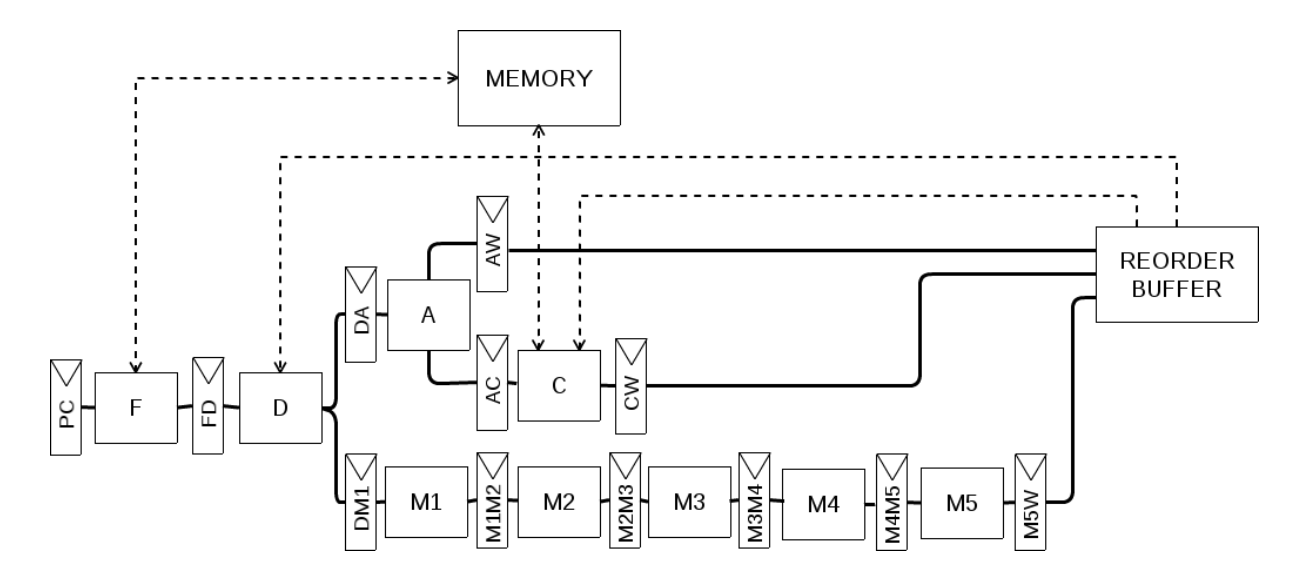
\includegraphics[width=0.8\textwidth]{inkel_pipeline}
    \caption{Pipeline general \emph{Inkel Pentium} extrasă din \cite{inkel}}
    \label{fig:inkel_pipeline}
\end{figure}

Varianta originală avea un cache de nivel 1 între procesor si memorie. Acest lucru se modifică pentru noua variantă.
Se adaugă un cache de nivel 2 comun pentru cele 2 core-uri și un circuit de arbitrare al accesului la bus. Aceste
modificări asupra structurii memoriei se pot vedea în figura \ref{fig:inkel_block_diagram}

\begin{figure}[h]
    \centering
    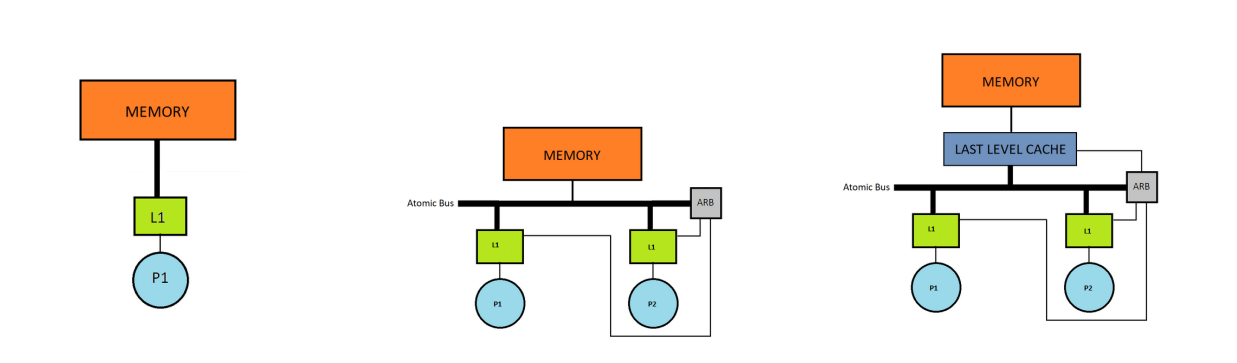
\includegraphics[width=0.8\textwidth]{inkel_block_diagram}
    \caption{Diagrama bloc cu evoluția structurii memoriei extrasă din \cite{inkel}}
    \label{fig:inkel_block_diagram}
\end{figure}

Coerența memoriei are legătură cu actualizarea datelor care sunt încărcate în cache-ul mai multor core-uri simultan.
Considerând un scenariu simplu în care Core A și Core B au același bloc de memorie în cache, iar Core A efectuează o
operatie de scriere în acest bloc, în această situație blocul de memorie din cache-ul aferent lui Core B conține informații
neactualizate, ca urmare apare un conflict ce poate duce la consecințe foarte grave. Pentru a rezolva problema coerenței
trebuie implementat un protocol de coerență. În lucrare au ales să folosească cel mai simplu protocol, protocolul \acrfull{vi},
care se comportă după cum arată diagrama de stare din figura \ref{fig:inkel_coherence}. Fiecare bloc de memorie din cache
se poate afla în una din cele 2 stări. Revenind la exemplul dat, acum blocul din cache-ul aferent lui Core B trece în
starea Invalid și va genera un \emph{cache miss} la citire sau scriere.

\begin{figure}[h]
    \centering
    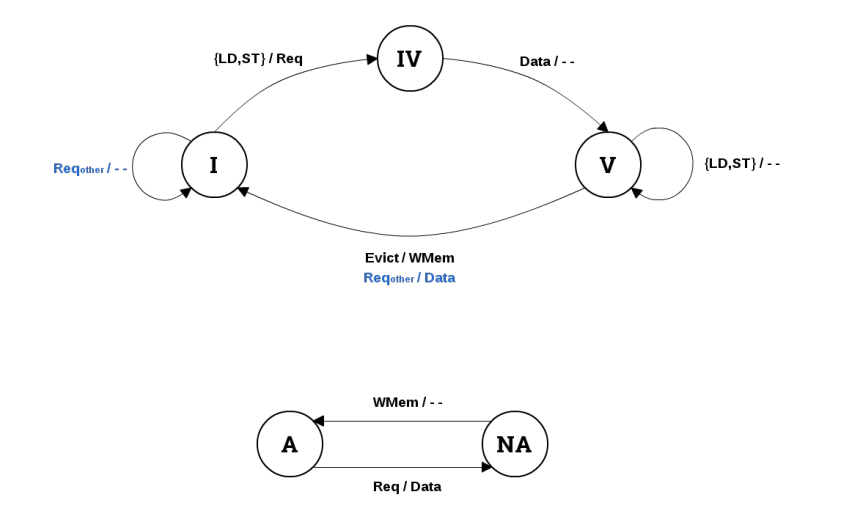
\includegraphics[width=0.8\textwidth]{inkel_coherence}
    \caption{Protocolul \acrshort{vi} extrasă din \cite{inkel}}
    \label{fig:inkel_coherence}
\end{figure}

\end{document}